% Generated by paper/export_memory_diagnostics_tikz.py.
% Requires \usepackage{pgfplots} and \pgfplotsset{compat=1.18}.
% Input inside a subfigure; do not resizebox the result (fonts would shrink).
\begingroup
\definecolor{diagKeep}{HTML}{4C8C4A}
\definecolor{diagFifo}{HTML}{D55E00}
\definecolor{diagUnbounded}{HTML}{4D4D4D}
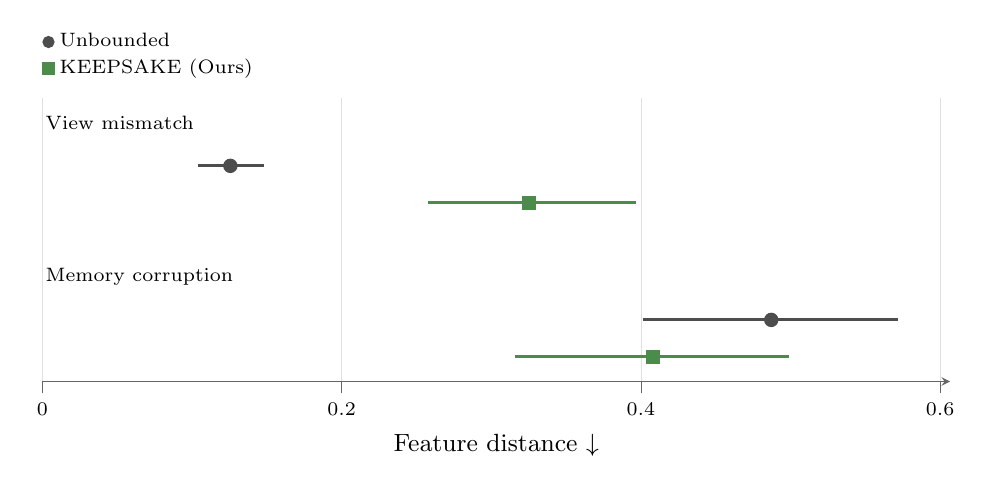
\begin{tikzpicture}
% Matched 60-s / 15-trajectory comparison; common baseline pixels.
\begin{axis}[
  scale only axis, width=\dimexpr\linewidth-17pt\relax, height=36mm,
  xmin=0.000000, xmax=0.606633, ymin=-0.28, ymax=1.56,
  ytick=\empty, xtick distance=0.2, scaled ticks=false,
  tick label style={font=\scriptsize}, label style={font=\small},
  xlabel={Feature distance $\downarrow$}, axis lines=left,
  y axis line style={draw=none}, axis line style={black!60}, tick style={black!60},
  tick align=outside, xmajorgrids=true, grid style={black!12,line width=0.25pt},
  clip=false, enlargelimits=false,
  legend style={font=\scriptsize,draw=none,fill=none,at={(0,1.05)},anchor=south west,
                legend columns=1,inner sep=0pt,row sep=-1pt},
  legend cell align=left,
]
\addlegendimage{only marks,mark=*,diagUnbounded}
\addlegendentry{Unbounded}
\addlegendimage{only marks,mark=square*,diagKeep}
\addlegendentry{KEEPSAKE (Ours)}
\node[anchor=west,font=\scriptsize,inner sep=1pt,fill=white]
  at (axis cs:0.000000,1.40) {View mismatch};
\node[anchor=west,font=\scriptsize,inner sep=1pt,fill=white]
  at (axis cs:0.000000,0.40) {Memory corruption};
\draw[diagUnbounded,line width=1.1pt] (axis cs:0.104065,1.12) -- (axis cs:0.147862,1.12);
\addplot[only marks,diagUnbounded,mark=*,mark size=2.4pt]
  coordinates {(0.125602,1.12)};
\draw[diagUnbounded,line width=1.1pt] (axis cs:0.401161,0.12) -- (axis cs:0.571633,0.12);
\addplot[only marks,diagUnbounded,mark=*,mark size=2.4pt]
  coordinates {(0.487087,0.12)};
\draw[diagKeep,line width=1.1pt] (axis cs:0.257853,0.88) -- (axis cs:0.396434,0.88);
\addplot[only marks,diagKeep,mark=square*,mark size=2.4pt]
  coordinates {(0.325372,0.88)};
\draw[diagKeep,line width=1.1pt] (axis cs:0.315901,-0.12) -- (axis cs:0.498888,-0.12);
\addplot[only marks,diagKeep,mark=square*,mark size=2.4pt]
  coordinates {(0.407863,-0.12)};
\end{axis}
\end{tikzpicture}
\endgroup
